\documentclass[10pt]{article}
\usepackage[utf8]{inputenc}
\usepackage[T1]{fontenc}
\usepackage{amsmath}
\usepackage{amsfonts}
\usepackage{amssymb}
\usepackage[version=4]{mhchem}
\usepackage{stmaryrd}
\usepackage{bbold}

\title{Instructions: }

\author{}
\date{}

\usepackage{tikz,graphicx,amsmath,amsfonts,amscd,amssymb,bm,cite,epsfig,epsf,url}
\begin{document}
\maketitle
\begin{itemize}
  \item Upload your submission to Gradescope. There, indicate the page on which each problem is written.

  \item Unless otherwise stated, all answers must be mathematically justified.

  \item Partial answers will be graded.

  \item You may discuss with other students, but you must write your own solutions separately based on your own understanding. List the students you work with (this won`t affect your grade).

  \item If you have questions, please feel free to ask on Piazza (rather than email) or at the office hours of the section leaders or instructor. Piazza sign-up link: piazza. com/nyu/fall2022/dsga1014

\end{itemize}

Problem $11.1$ (8 points). For the following functions, compute all critical points and determine if they are saddle points or local minimizers/maximizers.

(a) $f: \mathbb{R} \rightarrow \mathbb{R}$ where $f(x)=\left(x^{2}-1\right)^{2}+2022$.
\begin{itemize}
    \item for a function in $\mathbb{R}$ we know that critical points are points such that $f'(x)=0$
    \item in this case we know that $f'(x)=2(x^2-1)(2x)=4x^3-4x$
    \item so the critical points are x such that $=2(x^2-1)(2x)=0$ and thus we have x=-1, 1, or 0
    \item as $f''(x)=12x^2-4$ we can see that
    \item $f''(0)=-4$ meaning that 0 is a local max 
    \item $f''(-1)=12(1)-4=8$ so it is a local min
    \item $f''(1)=12(1)-4=8$ so it is a local min
\end{itemize}
(b) $g: \mathbb{R}^{3} \rightarrow \mathbb{R}$ where $g(x, y, z)=x^{2}+y^{2}+z^{2}-6 x+10 y-2 z$.
\begin{itemize}
    \item ok so we know that our critical points will have gradient equal to zero
    \item so we can solve for the gradient as $\nabla f_(x)=\begin{pmatrix}2x-6\\2y+10\\2z-2\end{pmatrix}$
    \item the only case that will solve all these equations is the vector \begin{pmatrix}3\\-5\\1\end{pmatrix}
    \item then to check what type of extrema this point is we need to look at the hessian matrix 
    $H_{f(X)}=$\begin{pmatrix}2&0&0\\0&2&0\\0&0&2\end{pmatrix} for all values of x 
    \item we can see that this matrix is just 2 times the identity matrix and thus will have all eigen values of 2, thus it is positive definite and the point  \begin{pmatrix}3\\-5\\1\end{pmatrix} is a local minima 
\end{itemize}
\newpage
Problem 11.2 (6 points). Same as above, but now for the more complicated function $h: \mathbb{R}^{3} \rightarrow \mathbb{R}$ where $h(x, y, z)=\left(x^{2}-z^{2}\right) y-3$ which, as you will see, has infinitely many critical points.

(a) Compute the gradient and Hessian of $h$.
\begin{itemize}
    \item let us first find the gradient 
    \item we know that $\nabla f(x)=\begin{pmatrix}
        2xy\\x^2-z^2\\-2zy
    \end{pmatrix}$
    \item now we can find the hessian
    \item $H_{f_(x)}=$\begin{pmatrix}2y&2x&0\\2x&0&-2z\\0&-2z&-2y\end{pmatrix}
\end{itemize}

(b) Show that the critical points are precisely the points of the form (i) $\{(0, t, 0): t \in \mathbb{R}\}$, or (ii) $\{(t, 0, t): t \in \mathbb{R}\}$, or (iii) $\{(t, 0,-t): \mathbb{R}\}$.
\begin{itemize}
    \item we know that a critical point x must satisfy $\nabla f_(x)=0$
    \item suppose for the sake of contradiction that there is a critical point x that is of none of the proposed forms. 
    \item case 1 
    \begin{itemize}
        \item suppose x=0
        \item if this is the case we know that $\nabla f(x)=\begin{pmatrix}
        -2xy\\x^2-z^2\\2xy
    \end{pmatrix}=\begin{pmatrix}
        0\\0-z^2\\-2zy
    \end{pmatrix}=0$
    \item we know that $-z^2=0$ only holds for z=0, and this will hold for any value of y. \item thus a critical point with an x=0 must take the from $\{(0, t, 0): t \in \mathbb{R}\}$
    \end{itemize}
    \item case 2
    \begin{itemize}
        \item suppose $x\neq 0$ then we have 
         $\nabla f(x)=\begin{pmatrix}
        2xy\\x^2-z^2\\-2zy
    \end{pmatrix}=0$  2xy=0 and 2zy=0 can both be satisfied regardless of the values of x and z as long as y=0
    \item now it must also be the case that $x^2-z^2=0$ this holds if $x^2=z^2$ which holds if x=-z or x=z
    \item thus the critical points of f with $x\neq 0$ must take the form $\{(t, 0, t): t \in \mathbb{R}\}$ $\{(t, 0,-t): \mathbb{R}\}$.
    \end{itemize}
    \item thus we have covered all possible types of critical points for the function f and shown they must be of these solutions.
\end{itemize}
(c) For all non-zero critical points, determine if they are saddle points or local minimizers/maximizers. (Ignore zero since there the Hessian vanishes, and when that happens one needs higher-order derivative information to determine if it is a saddle point or local minimizer/maximizer.) Hint: you may use without proof the fact that the matrices

$$
A:=\left[\begin{array}{ccc}
0 & 1 & 0 \\
1 & 0 & -1 \\
0 & -1 & 0
\end{array}\right] \text { and } B:=\left[\begin{array}{lll}
0 & 1 & 0 \\
1 & 0 & 1 \\
0 & 1 & 0
\end{array}\right]
$$

both have the same set of eigenvalues: $\sqrt{2},-\sqrt{2}, 0$.
\begin{itemize}
    \item from part a we know that $H_{f_(x)}=\begin{pmatrix}2y&2x&0\\2x&0&-2z\\0&-2z&-2y\end{pmatrix}$
    \item case 1 $v=(0,t,0)^T$
    \begin{itemize}
        \item $H_{f_(v)}=\begin{pmatrix}2t&0&0\\0&0&0\\0&0&-2t\end{pmatrix}$
        \item we can further see that \begin{pmatrix}
            1\\0\\0
        \end{pmatrix}\begin{pmatrix}2t&0&0\\0&0&0\\0&0&-2t\end{pmatrix}=\begin{pmatrix}
            2y\\0\\0
        \end{pmatrix}=2t\begin{pmatrix}
            1\\0\\0
        \end{pmatrix} thus the hessian has an eigen value of 2t. 

     \item we can further see that \begin{pmatrix}
            0\\1\\0
        \end{pmatrix}\begin{pmatrix}2t&0&0\\0&0&0\\0&0&-2t\end{pmatrix}=\begin{pmatrix}
            0\\0\\0
        \end{pmatrix}=0\begin{pmatrix}
            0\\1\\0
        \end{pmatrix} thus the hessian has an eigen value of 0. 
     \item we can further see that \begin{pmatrix}
            0\\0\\1
        \end{pmatrix}\begin{pmatrix}2t&0&0\\0&0&0\\0&0&-2t\end{pmatrix}=\begin{pmatrix}
            0\\0\\-2t
        \end{pmatrix}=-2t\begin{pmatrix}
            1\\0\\0
        \end{pmatrix} thus the hessian has an eigen value of -2t. 
    \item so for all non zero values of t, our hessian will have one postive one zero and one negative eigen value and thus we can say these will all be saddle points 
\end{itemize}
\item case 2  $v=(t,0,t)^T$
\begin{itemize}
    \item in this case our hessian becomes   \item $H_{f_(x)}=$\begin{pmatrix}2y&2x&0\\2x&0&-2z\\0&-2z&-2y\end{pmatrix}=\begin{pmatrix}0&2t&0\\2t&0&-2t\\0&-2t&0\end{pmatrix}=2tA where A is the matrix from the problem description 
    \item thus we know that our hessian will have eigen values equal to $2t\sqrt{t}, -2t\sqrt{2},0$
        \item so for all non zero values of t, our hessian will have one positive one zero and one negative eigen value and thus we can say these will all be saddle points 
\end{itemize}
\item case 2  $v=(t,0,-t)^T$
\begin{itemize}
    \item in this case our hessian becomes   \item $H_{f_(x)}=$\begin{pmatrix}2y&2x&0\\2x&0&-2z\\0&-2z&-2y\end{pmatrix}=\begin{pmatrix}0&2t&0\\2t&0&2t\\0&2t&0\end{pmatrix}=2tB where B is the matrix from the problem description 
    \item thus we know that our hessian will have eigen values equal to $2t\sqrt{t}, -2t\sqrt{2},0$
        \item so for all non zero values of t, our hessian will have one positive one zero and one negative eigen value and thus we can say these will all be saddle points 
\end{itemize}


\end{itemize}





\newpage

Problem 11.3 (6 points). Consider the following constrained optimization problem in $\mathbb{R}^{2}$ :

$$
\text { minimize } x^{2}+y^{2} \quad \text { subject to } \quad 2 x+y=4 .
$$

You may use without proof the fact that this minimization problem has at least one solution. (This comes from the general fact that a continuous function on a compact set has a minimizer.)

(a) Using Lagrange multipliers, show that (1) has a unique solution and compute its coordinates.
\begin{itemize}
    \item we know that our critical point must have the form $\nabla f(x,y)+\lambda \nabla g(x)=0$
    \item we know that $\nabla f_(x,y)=\begin{pmatrix}
        2x\\2y
    \end{pmatrix}$
    \item we can also write our constrain g(X)=2x+y-4=0 which has gradient $\nabla g(X)=\begin{pmatrix}
        2\\1
    \end{pmatrix}$
    \item so thus we have  $0=\nabla f(x,y)+\lambda \nabla g(x)=\begin{pmatrix}
        2x\\2y
    \end{pmatrix}+\begin{pmatrix}
        \lambda 2\\\lambda 1\end{pmatrix}$ 
        \item we can see clearly $\lambda=0$ is not valid 
        \item so if $\lambda\neq 0$ we can say  this equation is solved by x such that $x=\begin{pmatrix}
        -\lambda\\-\frac{\lambda}{2} \end{pmatrix}$
        \item then we can plug this into our constraint to get the value of $\lambda$ $g(\begin{pmatrix}
            -\lambda\\\frac{1}{2}\lambda 
        \end{pmatrix})=-2\lambda -\frac{-\lambda}{2}=4$ whcih yields $\lambda=-\frac{8}{5}$
        \item and finally a sollution $x=\begin{pmatrix}
        \frac{8}{5}\\\frac{8}{10} \end{pmatrix}$
        \item and plugging this sollution into our objective yields f(x,y)=3.2
\end{itemize}
\newline
\\ 
\\

(b) Draw a picture in $\mathbb{R}^{2}$ representing the problem. Specifically, draw the solution, the constraint set, the gradient of the objective as a vector emanating from the solution, and three contour lines for the objective - the contours with values 2, 8, and the optimal value.
\begin{itemize}
    \item 

 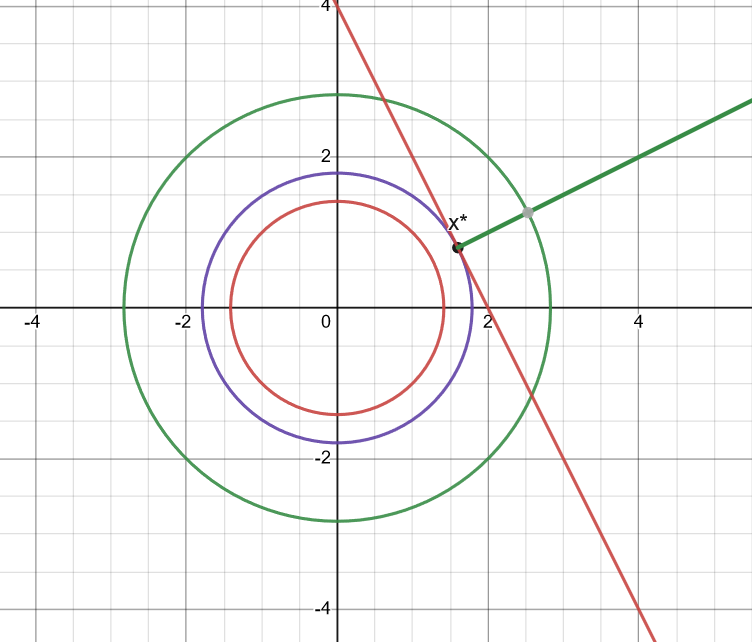
\includegraphics[width=10cm]{homework 11/homework 11 question 3c.png}
\end{itemize}
\end{document}